\section{Differential Evolution}
DE is a population-based optimization algorithm, where operators for mutation, crossover, and selection act to create a new population from an existing one. Eventually, through a series of iterations, the population will converge on to a globally optimal solution \cite{Poole3}. The DE is suitable for problems with discontinuous objectives, also with a problem having multiple local optima (multimodality). However, DE has slow convergence. Nearly 200 times more functional evaluations are required for Gradient-free methods as compared to gradient-based methods \cite{oleg}.

The DE is a parallel direct search method which utilizes $N$
D-dimensional design vectors \textbf{x$_{n,G}$}, where n = 1, 2, ... , N and g is the generation ranging between $[1, G]$. $N$ does not alter during the optimization
process. The initial population is chosen randomly and should cover the entire design space. As a rule, it is assumed to follow a uniform probability distribution for all random decisions unless otherwise stated. In case a preliminary solution is available, the initial population might be generated by adding normal distributed random deviations to the nominal solution $\textbf{x}_{nom,0}$. The DE generates another vectors by adding the weighted difference between two population vectors to a third vector. This operation is called \textit{mutation}.

The mutated vector individuals are merged with the individuals of another predetermined vector, the target vector, to generate the \textit{trial vector}. This operation is referred to as "\textit{crossover}." If the trial vector yields a lower cost function value than the target vector, the trial vector replaces the target vector in the following generation. This last operation is called "\textit{selection}". Each population vector has to serve once as the target vector so that $ N $ competitions occur in a given generation \cite{storn}.

The mathematical representation of the DE algorithm is explained as follows.
\begin{enumerate}
\item \underline{Initialization}: Here the initial population $N$ is generated randomly as: 
\begin{equation}
\textbf{x}_{n,g}^{d}=\textbf{L}^{d}+\operatorname{rand}(0,1)\left(\textbf{U}^{d}-\textbf{L}^{d}\right)
\label{initlize}
\end{equation}
where $rand(0, 1)$ is a uniformly distributed random number on the interval [0, 1]. $L^d$ and $U^d$ represents the lower and the upper limits of the design space respectively. And, $d$ is dimension of problem which can be $(d\in\{1, \ldots, D\}))$.

\item \underline{Mutation}: For each individual in the population, corresponding donor vector is generated as follows: initially, the weighted difference is taken between two randomly selected individuals from population,then it is added it to base vector (\textbf{x}$_{b,G}$). There are several strategies proposed that define the base vector. If in case DE/best/1 strategy is chosen, then the \(n\)-th donor vector is represented using equation \ref{best_mutation}. 
\begin{equation}
\mathbf{v}_{n}=\mathbf{x}_{b}(t)+F\left(\mathbf{x}_{r_{1}}(t)-\mathbf{x}_{r_{2}}(t)\right)
\label{best_mutation}
\end{equation}
$$
b=\underset{i \in\{1, \ldots, N\}}{\arg \min } f\left(\mathbf{x}_{i}\right)
$$
where, $F$ is the scaling factor ranging between [0, 1]. A higher scaling factor may force the donor individual to fall out of design space. Whereas, the lower value will generate the donor vector close to target individual. A value of $F = 0.5$ is considered to be a good trade off. $x_{b,g-1}$ is the best individual from the previous generation. $r_1$ and $r_2$ are uniformly distributed random integers in the interval [1, N] such that \(r_{1} \neq r_{2} \neq b\) and \(r_{1} \neq r_{2} \neq n\). A better representation of mutation stage in 2-D design space is shown in figure \ref{mutation}.
\begin{figure}[!ht]
    \centering
    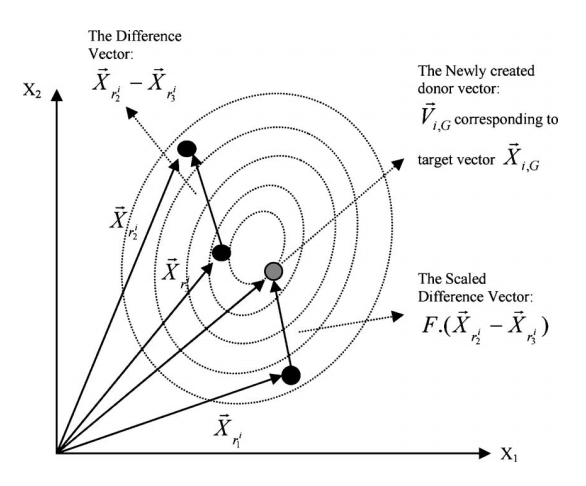
\includegraphics[scale = 0.5]{figures/mutation.png}
    \caption{2-D design space representing mutation stage \cite{storn}.}
    \label{mutation}
\end{figure}

\item \underline{Cross-over}: In this stage, elements from the target vector and donor vector are combined in a specific order to get a trial vector (\textbf{u}$_{n,g}$). This process is referred as binomial crossover. This stage play a vital role in increasing the population's diversity, and is shown in equation \ref{cross-over}.

\begin{figure}[!ht]
    \centering
    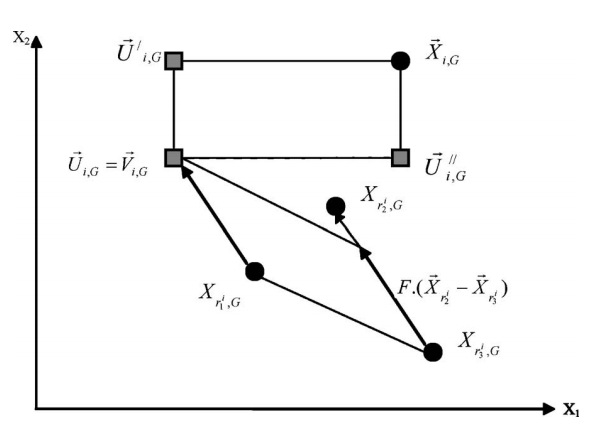
\includegraphics[scale = 0.5]{figures/crossover.png}
    \caption{Different possible trial vector formed due to Uniform/Binomial crossover between mutant vector and target vector in 2-D design space\cite{storn}.}
    \label{crossover}
\end{figure}

\begin{equation}
\mathbf{u}_{n,g}=\left\{\begin{array}{ll}{\mathbf{v}_{n,g}} & {\text { if rand }(0,1) \leq C R \text { or } r_{n}=d} \\ {\mathbf{x}_{n,g}} & {\text { otherwise }}\end{array}\right.
\label{cross-over}
\end{equation}
where $r_n$ is the uniformly distributed random integer in the interval [1, D], and $CR$ is the crossover probability. $CR = 1$ implies there is no diversity, meaning the parent individuals are not carried to the next generation. On the other hand, $CR = 0$ implies that all generated elements are the same as parent elements, so there is no evolution over generations.

\item \underline{Selection}: The trial individuals and target individuals are compared based on their function values. During the problem with the minimization case, an individual with minimum function value is retained. On the other hand, for maximization problems, an individual with a maximum function value is retained. Equation \ref{selection} represents the selection phase.
\begin{equation}
\mathbf{x}_{n}(t+1)=\left\{\begin{array}{ll}{\mathbf{u}_{n}} & {\text { if } f\left(\mathbf{u}_{n}\right) \leq f\left(\mathbf{x}_{n}(t)\right)} \\ {\mathbf{x}_{n}(t)} & {\text { otherwise }}\end{array}\right.
\label{selection}
\end{equation}

\item \underline{Stopping condition}: The optimization can have single or multiple stopping conditions, like the maximum number of function evaluations, epsilon value, to name a few. The author D.J.Poole used the maximum number of function evaluations ($FEs_{max}$) as the stopping condition for all the algorithms.
\end{enumerate}

The algorithm \ref{DE algorithm} depicts the pseudo-code for the DE algorithm.
\begin{algorithm}[!ht]
\SetAlgoNoLine
 Randomly initialise individuals and calculate objective\\
 \While{\text { $FEs <FEs_{max}$ }}
 {
  \For{$n=1 \rightarrow N$}
  {
  Perform mutation: equation \ref{best_mutation}\\
  Perform binomial crossover: equation \ref{cross-over}\\
  Calculate objective and constraints of trial vector
  }
  \For{$n=1 \rightarrow N$}{
 Update $n$-th target vector: equation \ref{selection}
 }
 }
 \caption{DE algorithm}
 \label{DE algorithm}
\end{algorithm}

In the next section, details about mutation strategies are explained. 

\section{DE Strategies}
In the DE algorithm, there are different variants for the mutation stage. Some of these are mentioned in the upcoming subsections \cite{chi}.

\subsection{DE/rand/1}
In this strategy, the mutation stage is carried out by taking single pair of the weighted difference. The individuals involved are randomly selected from the populations, Further, the weighted difference is added to base individual resulting in target vector as shown in equation \ref{DE-rand-1}.
\begin{equation}
    \mathbf{v}_{n, g}=\mathbf{x}_{r_{1}, g}+F.\left(\mathbf{x}_{r_{2}, g}-\mathbf{x}_{r_{3}, g}\right)
    \label{DE-rand-1}
\end{equation}

\subsection{DE/best/1}
This method work the same way as DE/rand/1 strategy, except that it generates the individual base vector $x_{b}$ as in equation \ref{DE-best-1}.
\begin{equation}
    \mathbf{v}_{n, g}=\mathbf{x}_{b, g-1}+F.\left(\mathbf{x}_{r_{1}, g}-\mathbf{x}_{r_{2}, g}\right)
    \label{DE-best-1}
\end{equation}
where,
$$
b=\underset{i \in\{1, \ldots, N\}}{\arg \min } f\left(\mathbf{x}_{i, g-1}\right)
$$

\subsection{DE/best/2}
This strategy involve evaluating the mutant vector with two weighted ($F_1, F_2$) differences of vectors which are picked randomly from the population size \(N\), and added to base vector (best) \(x_b\). Equation \ref{DE-best-2} represents the same.
\begin{equation}
  \mathbf{v}_{n, g}=\mathbf{x}_{b, g-1}
+F_{1}.\left(\mathbf{x}_{r_{1}, g}-\mathbf{x}_{r_{2}, g}\right)
+F_{2}.\left(\mathbf{x}_{r_{3}, g}-\mathbf{x}_{r_{4}, g}\right)
\label{DE-best-2}
\end{equation}
where,
$$
b=\underset{i \in\{1, \ldots, N\}}{\arg \min } f\left(\mathbf{x}_{i, g}\right)
$$

\subsection{DE/current to best/2}
In this strategy, one of the two weighted differences will take place between the best vector and the vector index for which perturbation is carried out. Equation \ref{DE-ctob-2} depicts the above strategy. 
$$\mathbf{v}_{n}=\mathbf{x}_{b}(t)
+F_{1}\left(\mathbf{x}_{r_{1}}(t)-\mathbf{x}_{r_{2}}(t)\right)
+F_{2}\left(\mathbf{x}_{b}(t)-\mathbf{x}_{r_n}(t)\right)$$
where,
$$
b=\underset{i \in\{1, \ldots, N\}}{\arg \min } f\left(\mathbf{x}_{i}\right)
$$

\subsection{DE/rand/2}
This strategy involve two weighted differences between individuals. These individuals are randomly selected in the given population. Equation \ref{DE-rand-2} represents the mutant vector generation using the DE/rand/2 strategy. 
$$\mathbf{v}_{n}=\mathbf{x}_{r_{1}}(t)
+F_{1}\left(\mathbf{x}_{r_{2}}(t)-\mathbf{x}_{r_{3}}(t)\right)
+F_{2}\left(\mathbf{x}_{r_{4}}(t)-\mathbf{x}_{r_{5}}(t)\right)$$
where, $r_1, r_2, r_3, r_4, r_5 \in [1, NP]$ and $\neq$ running index $i$. 


\subsection{Comparision between strategies}
The author H.Chi \cite{chi} mention that the strategies like \textit{DE/best/1}, \textit{DE/best/2} and \textit{DE/current to best/2} can improve the convergence rate of DE, and converge in the local optimal due to usage of the best vector. On the other hand, \textit{DE/rand/2} and \textit{DE/rand/1} relatively enhance the convergence rate of finding the global optimal but have slow convergence speed. Several test functions like Sphere function, Rosenbock's function, Step function, Quartic function, etc. are tested using the Niching algorithm, and results obtained coincide with the actual optimal values. Chapter \ref{results} highlights more on test function results.